% Created by tikzDevice version 0.10.1 on 2017-11-29 19:14:38
% !TEX encoding = UTF-8 Unicode
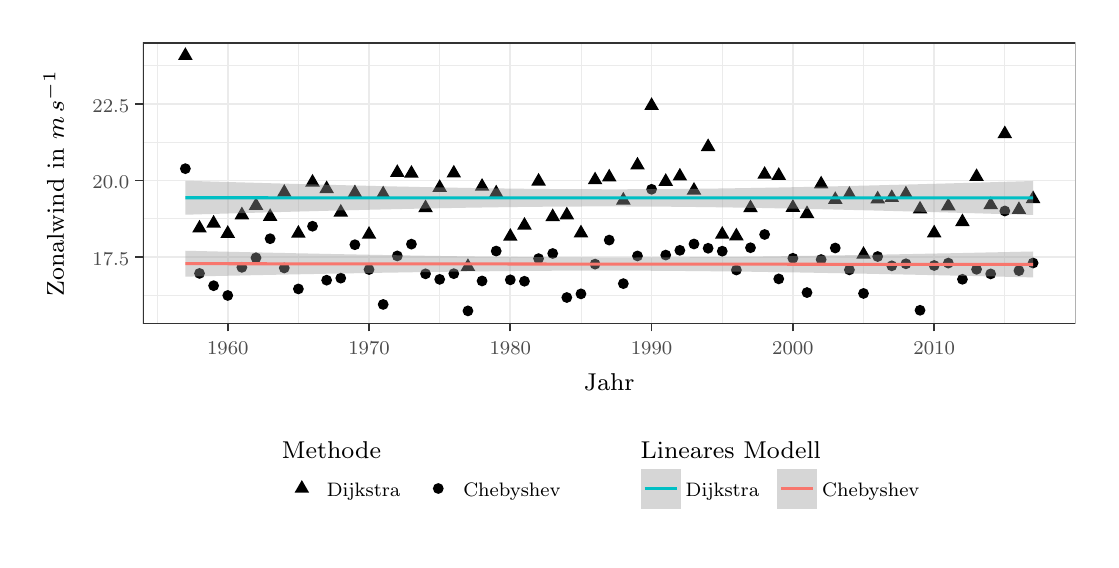
\begin{tikzpicture}[font=\footnotesize,x=1pt,y=1pt]
\definecolor{fillColor}{RGB}{255,255,255}
\path[use as bounding box,fill=fillColor,fill opacity=0.00] (0,0) rectangle (384.11,184.94);
\begin{scope}
\path[clip] (  0.00,  0.00) rectangle (384.11,184.94);
\definecolor{drawColor}{RGB}{255,255,255}
\definecolor{fillColor}{RGB}{255,255,255}

\path[draw=drawColor,line width= 0.6pt,line join=round,line cap=round,fill=fillColor] (  0.00,  0.00) rectangle (384.11,184.94);
\end{scope}
\begin{scope}
\path[clip] ( 41.67, 77.99) rectangle (378.61,179.44);
\definecolor{fillColor}{RGB}{255,255,255}

\path[fill=fillColor] ( 41.67, 77.99) rectangle (378.61,179.44);
\definecolor{drawColor}{gray}{0.92}

\path[draw=drawColor,line width= 0.3pt,line join=round] ( 41.67, 88.30) --
	(378.61, 88.30);

\path[draw=drawColor,line width= 0.3pt,line join=round] ( 41.67,115.91) --
	(378.61,115.91);

\path[draw=drawColor,line width= 0.3pt,line join=round] ( 41.67,143.52) --
	(378.61,143.52);

\path[draw=drawColor,line width= 0.3pt,line join=round] ( 41.67,171.13) --
	(378.61,171.13);

\path[draw=drawColor,line width= 0.3pt,line join=round] ( 46.77, 77.99) --
	( 46.77,179.44);

\path[draw=drawColor,line width= 0.3pt,line join=round] ( 97.82, 77.99) --
	( 97.82,179.44);

\path[draw=drawColor,line width= 0.3pt,line join=round] (148.88, 77.99) --
	(148.88,179.44);

\path[draw=drawColor,line width= 0.3pt,line join=round] (199.93, 77.99) --
	(199.93,179.44);

\path[draw=drawColor,line width= 0.3pt,line join=round] (250.98, 77.99) --
	(250.98,179.44);

\path[draw=drawColor,line width= 0.3pt,line join=round] (302.03, 77.99) --
	(302.03,179.44);

\path[draw=drawColor,line width= 0.3pt,line join=round] (353.09, 77.99) --
	(353.09,179.44);

\path[draw=drawColor,line width= 0.3pt,line join=round] (378.61, 77.99) --
	(378.61,179.44);

\path[draw=drawColor,line width= 0.6pt,line join=round] ( 41.67,102.11) --
	(378.61,102.11);

\path[draw=drawColor,line width= 0.6pt,line join=round] ( 41.67,129.72) --
	(378.61,129.72);

\path[draw=drawColor,line width= 0.6pt,line join=round] ( 41.67,157.33) --
	(378.61,157.33);

\path[draw=drawColor,line width= 0.6pt,line join=round] ( 72.30, 77.99) --
	( 72.30,179.44);

\path[draw=drawColor,line width= 0.6pt,line join=round] (123.35, 77.99) --
	(123.35,179.44);

\path[draw=drawColor,line width= 0.6pt,line join=round] (174.40, 77.99) --
	(174.40,179.44);

\path[draw=drawColor,line width= 0.6pt,line join=round] (225.45, 77.99) --
	(225.45,179.44);

\path[draw=drawColor,line width= 0.6pt,line join=round] (276.51, 77.99) --
	(276.51,179.44);

\path[draw=drawColor,line width= 0.6pt,line join=round] (327.56, 77.99) --
	(327.56,179.44);
\definecolor{fillColor}{RGB}{0,0,0}

\path[fill=fillColor] ( 56.98,133.99) circle (  1.96);

\path[fill=fillColor] ( 62.09, 96.14) circle (  1.96);

\path[fill=fillColor] ( 67.19, 91.70) circle (  1.96);

\path[fill=fillColor] ( 72.30, 88.17) circle (  1.96);

\path[fill=fillColor] ( 77.40, 98.33) circle (  1.96);

\path[fill=fillColor] ( 82.51,101.78) circle (  1.96);

\path[fill=fillColor] ( 87.61,108.68) circle (  1.96);

\path[fill=fillColor] ( 92.72, 98.11) circle (  1.96);

\path[fill=fillColor] ( 97.82, 90.53) circle (  1.96);

\path[fill=fillColor] (102.93,113.19) circle (  1.96);

\path[fill=fillColor] (108.03, 93.69) circle (  1.96);

\path[fill=fillColor] (113.14, 94.43) circle (  1.96);

\path[fill=fillColor] (118.24,106.51) circle (  1.96);

\path[fill=fillColor] (123.35, 97.54) circle (  1.96);

\path[fill=fillColor] (128.46, 84.93) circle (  1.96);

\path[fill=fillColor] (133.56,102.46) circle (  1.96);

\path[fill=fillColor] (138.67,106.72) circle (  1.96);

\path[fill=fillColor] (143.77, 95.99) circle (  1.96);

\path[fill=fillColor] (148.88, 93.99) circle (  1.96);

\path[fill=fillColor] (153.98, 96.05) circle (  1.96);

\path[fill=fillColor] (159.09, 82.60) circle (  1.96);

\path[fill=fillColor] (164.19, 93.41) circle (  1.96);

\path[fill=fillColor] (169.30,104.22) circle (  1.96);

\path[fill=fillColor] (174.40, 93.82) circle (  1.96);

\path[fill=fillColor] (179.51, 93.31) circle (  1.96);

\path[fill=fillColor] (184.61,101.49) circle (  1.96);

\path[fill=fillColor] (189.72,103.34) circle (  1.96);

\path[fill=fillColor] (194.82, 87.43) circle (  1.96);

\path[fill=fillColor] (199.93, 88.75) circle (  1.96);

\path[fill=fillColor] (205.03, 99.49) circle (  1.96);

\path[fill=fillColor] (210.14,108.19) circle (  1.96);

\path[fill=fillColor] (215.24, 92.45) circle (  1.96);

\path[fill=fillColor] (220.35,102.45) circle (  1.96);

\path[fill=fillColor] (225.45,126.53) circle (  1.96);

\path[fill=fillColor] (230.56,102.77) circle (  1.96);

\path[fill=fillColor] (235.67,104.48) circle (  1.96);

\path[fill=fillColor] (240.77,106.77) circle (  1.96);

\path[fill=fillColor] (245.88,105.23) circle (  1.96);

\path[fill=fillColor] (250.98,104.17) circle (  1.96);

\path[fill=fillColor] (256.09, 97.37) circle (  1.96);

\path[fill=fillColor] (261.19,105.42) circle (  1.96);

\path[fill=fillColor] (266.30,110.21) circle (  1.96);

\path[fill=fillColor] (271.40, 94.16) circle (  1.96);

\path[fill=fillColor] (276.51,101.61) circle (  1.96);

\path[fill=fillColor] (281.61, 89.22) circle (  1.96);

\path[fill=fillColor] (286.72,101.15) circle (  1.96);

\path[fill=fillColor] (291.82,105.32) circle (  1.96);

\path[fill=fillColor] (296.93, 97.42) circle (  1.96);

\path[fill=fillColor] (302.03, 88.90) circle (  1.96);

\path[fill=fillColor] (307.14,102.24) circle (  1.96);

\path[fill=fillColor] (312.24, 98.88) circle (  1.96);

\path[fill=fillColor] (317.35, 99.62) circle (  1.96);

\path[fill=fillColor] (322.45, 82.82) circle (  1.96);

\path[fill=fillColor] (327.56, 99.00) circle (  1.96);

\path[fill=fillColor] (332.67, 99.87) circle (  1.96);

\path[fill=fillColor] (337.77, 94.01) circle (  1.96);

\path[fill=fillColor] (342.88, 97.62) circle (  1.96);

\path[fill=fillColor] (347.98, 95.96) circle (  1.96);

\path[fill=fillColor] (353.09,118.70) circle (  1.96);

\path[fill=fillColor] (358.19, 97.15) circle (  1.96);

\path[fill=fillColor] (363.30, 99.90) circle (  1.96);

\path[fill=fillColor] ( 56.98,177.88) --
	( 59.62,173.31) --
	( 54.34,173.31) --
	cycle;

\path[fill=fillColor] ( 62.09,115.51) --
	( 64.73,110.94) --
	( 59.44,110.94) --
	cycle;

\path[fill=fillColor] ( 67.19,117.30) --
	( 69.83,112.72) --
	( 64.55,112.72) --
	cycle;

\path[fill=fillColor] ( 72.30,113.60) --
	( 74.94,109.02) --
	( 69.65,109.02) --
	cycle;

\path[fill=fillColor] ( 77.40,120.29) --
	( 80.05,115.71) --
	( 74.76,115.71) --
	cycle;

\path[fill=fillColor] ( 82.51,123.68) --
	( 85.15,119.10) --
	( 79.87,119.10) --
	cycle;

\path[fill=fillColor] ( 87.61,119.69) --
	( 90.26,115.12) --
	( 84.97,115.12) --
	cycle;

\path[fill=fillColor] ( 92.72,128.43) --
	( 95.36,123.85) --
	( 90.08,123.85) --
	cycle;

\path[fill=fillColor] ( 97.82,113.65) --
	(100.47,109.07) --
	( 95.18,109.07) --
	cycle;

\path[fill=fillColor] (102.93,132.10) --
	(105.57,127.53) --
	(100.29,127.53) --
	cycle;

\path[fill=fillColor] (108.03,129.75) --
	(110.68,125.17) --
	(105.39,125.17) --
	cycle;

\path[fill=fillColor] (113.14,121.26) --
	(115.78,116.69) --
	(110.50,116.69) --
	cycle;

\path[fill=fillColor] (118.24,128.26) --
	(120.89,123.69) --
	(115.60,123.69) --
	cycle;

\path[fill=fillColor] (123.35,113.26) --
	(125.99,108.68) --
	(120.71,108.68) --
	cycle;

\path[fill=fillColor] (128.46,127.86) --
	(131.10,123.28) --
	(125.81,123.28) --
	cycle;

\path[fill=fillColor] (133.56,135.61) --
	(136.20,131.03) --
	(130.92,131.03) --
	cycle;

\path[fill=fillColor] (138.67,135.33) --
	(141.31,130.75) --
	(136.02,130.75) --
	cycle;

\path[fill=fillColor] (143.77,122.86) --
	(146.41,118.28) --
	(141.13,118.28) --
	cycle;

\path[fill=fillColor] (148.88,130.17) --
	(151.52,125.60) --
	(146.23,125.60) --
	cycle;

\path[fill=fillColor] (153.98,135.39) --
	(156.62,130.81) --
	(151.34,130.81) --
	cycle;

\path[fill=fillColor] (159.09,101.62) --
	(161.73, 97.04) --
	(156.44, 97.04) --
	cycle;

\path[fill=fillColor] (164.19,130.60) --
	(166.83,126.03) --
	(161.55,126.03) --
	cycle;

\path[fill=fillColor] (169.30,128.20) --
	(171.94,123.62) --
	(166.65,123.62) --
	cycle;

\path[fill=fillColor] (174.40,112.53) --
	(177.04,107.95) --
	(171.76,107.95) --
	cycle;

\path[fill=fillColor] (179.51,116.55) --
	(182.15,111.98) --
	(176.87,111.98) --
	cycle;

\path[fill=fillColor] (184.61,132.48) --
	(187.26,127.90) --
	(181.97,127.90) --
	cycle;

\path[fill=fillColor] (189.72,119.65) --
	(192.36,115.07) --
	(187.08,115.07) --
	cycle;

\path[fill=fillColor] (194.82,120.27) --
	(197.47,115.70) --
	(192.18,115.70) --
	cycle;

\path[fill=fillColor] (199.93,113.77) --
	(202.57,109.19) --
	(197.29,109.19) --
	cycle;

\path[fill=fillColor] (205.03,132.94) --
	(207.68,128.36) --
	(202.39,128.36) --
	cycle;

\path[fill=fillColor] (210.14,133.97) --
	(212.78,129.39) --
	(207.50,129.39) --
	cycle;

\path[fill=fillColor] (215.24,125.61) --
	(217.89,121.04) --
	(212.60,121.04) --
	cycle;

\path[fill=fillColor] (220.35,138.29) --
	(222.99,133.72) --
	(217.71,133.72) --
	cycle;

\path[fill=fillColor] (225.45,159.81) --
	(228.10,155.23) --
	(222.81,155.23) --
	cycle;

\path[fill=fillColor] (230.56,132.39) --
	(233.20,127.81) --
	(227.92,127.81) --
	cycle;

\path[fill=fillColor] (235.67,134.29) --
	(238.31,129.72) --
	(233.02,129.72) --
	cycle;

\path[fill=fillColor] (240.77,129.19) --
	(243.41,124.62) --
	(238.13,124.62) --
	cycle;

\path[fill=fillColor] (245.88,144.94) --
	(248.52,140.37) --
	(243.23,140.37) --
	cycle;

\path[fill=fillColor] (250.98,113.26) --
	(253.62,108.68) --
	(248.34,108.68) --
	cycle;

\path[fill=fillColor] (256.09,112.68) --
	(258.73,108.10) --
	(253.44,108.10) --
	cycle;

\path[fill=fillColor] (261.19,122.86) --
	(263.83,118.29) --
	(258.55,118.29) --
	cycle;

\path[fill=fillColor] (266.30,134.93) --
	(268.94,130.35) --
	(263.65,130.35) --
	cycle;

\path[fill=fillColor] (271.40,134.54) --
	(274.04,129.96) --
	(268.76,129.96) --
	cycle;

\path[fill=fillColor] (276.51,123.00) --
	(279.15,118.42) --
	(273.86,118.42) --
	cycle;

\path[fill=fillColor] (281.61,120.73) --
	(284.26,116.15) --
	(278.97,116.15) --
	cycle;

\path[fill=fillColor] (286.72,131.46) --
	(289.36,126.88) --
	(284.08,126.88) --
	cycle;

\path[fill=fillColor] (291.82,125.83) --
	(294.47,121.26) --
	(289.18,121.26) --
	cycle;

\path[fill=fillColor] (296.93,127.71) --
	(299.57,123.13) --
	(294.29,123.13) --
	cycle;

\path[fill=fillColor] (302.03,106.02) --
	(304.68,101.44) --
	(299.39,101.44) --
	cycle;

\path[fill=fillColor] (307.14,126.05) --
	(309.78,121.47) --
	(304.50,121.47) --
	cycle;

\path[fill=fillColor] (312.24,126.53) --
	(314.89,121.95) --
	(309.60,121.95) --
	cycle;

\path[fill=fillColor] (317.35,127.82) --
	(319.99,123.24) --
	(314.71,123.24) --
	cycle;

\path[fill=fillColor] (322.45,122.39) --
	(325.10,117.81) --
	(319.81,117.81) --
	cycle;

\path[fill=fillColor] (327.56,113.75) --
	(330.20,109.18) --
	(324.92,109.18) --
	cycle;

\path[fill=fillColor] (332.67,123.52) --
	(335.31,118.94) --
	(330.02,118.94) --
	cycle;

\path[fill=fillColor] (337.77,117.81) --
	(340.41,113.23) --
	(335.13,113.23) --
	cycle;

\path[fill=fillColor] (342.88,134.13) --
	(345.52,129.56) --
	(340.23,129.56) --
	cycle;

\path[fill=fillColor] (347.98,123.96) --
	(350.62,119.39) --
	(345.34,119.39) --
	cycle;

\path[fill=fillColor] (353.09,149.60) --
	(355.73,145.03) --
	(350.44,145.03) --
	cycle;

\path[fill=fillColor] (358.19,122.20) --
	(360.83,117.62) --
	(355.55,117.62) --
	cycle;

\path[fill=fillColor] (363.30,126.14) --
	(365.94,121.56) --
	(360.65,121.56) --
	cycle;
\definecolor{fillColor}{RGB}{153,153,153}

\path[fill=fillColor,fill opacity=0.40] ( 56.98,104.33) --
	( 60.86,104.24) --
	( 64.74,104.15) --
	( 68.61,104.06) --
	( 72.49,103.97) --
	( 76.37,103.88) --
	( 80.25,103.79) --
	( 84.12,103.71) --
	( 88.00,103.62) --
	( 91.88,103.54) --
	( 95.76,103.45) --
	( 99.63,103.37) --
	(103.51,103.29) --
	(107.39,103.20) --
	(111.27,103.12) --
	(115.14,103.05) --
	(119.02,102.97) --
	(122.90,102.89) --
	(126.78,102.82) --
	(130.65,102.75) --
	(134.53,102.68) --
	(138.41,102.61) --
	(142.28,102.54) --
	(146.16,102.48) --
	(150.04,102.42) --
	(153.92,102.36) --
	(157.79,102.30) --
	(161.67,102.25) --
	(165.55,102.20) --
	(169.43,102.15) --
	(173.30,102.11) --
	(177.18,102.07) --
	(181.06,102.03) --
	(184.94,102.00) --
	(188.81,101.97) --
	(192.69,101.94) --
	(196.57,101.92) --
	(200.45,101.91) --
	(204.32,101.89) --
	(208.20,101.89) --
	(212.08,101.88) --
	(215.96,101.88) --
	(219.83,101.89) --
	(223.71,101.90) --
	(227.59,101.91) --
	(231.46,101.93) --
	(235.34,101.95) --
	(239.22,101.98) --
	(243.10,102.01) --
	(246.97,102.04) --
	(250.85,102.08) --
	(254.73,102.12) --
	(258.61,102.16) --
	(262.48,102.21) --
	(266.36,102.26) --
	(270.24,102.31) --
	(274.12,102.37) --
	(277.99,102.42) --
	(281.87,102.48) --
	(285.75,102.54) --
	(289.63,102.61) --
	(293.50,102.67) --
	(297.38,102.74) --
	(301.26,102.81) --
	(305.14,102.88) --
	(309.01,102.95) --
	(312.89,103.02) --
	(316.77,103.10) --
	(320.65,103.17) --
	(324.52,103.25) --
	(328.40,103.33) --
	(332.28,103.40) --
	(336.15,103.48) --
	(340.03,103.56) --
	(343.91,103.65) --
	(347.79,103.73) --
	(351.66,103.81) --
	(355.54,103.89) --
	(359.42,103.98) --
	(363.30,104.06) --
	(363.30, 94.70) --
	(359.42, 94.79) --
	(355.54, 94.88) --
	(351.66, 94.97) --
	(347.79, 95.06) --
	(343.91, 95.15) --
	(340.03, 95.24) --
	(336.15, 95.32) --
	(332.28, 95.41) --
	(328.40, 95.49) --
	(324.52, 95.58) --
	(320.65, 95.66) --
	(316.77, 95.74) --
	(312.89, 95.82) --
	(309.01, 95.90) --
	(305.14, 95.98) --
	(301.26, 96.06) --
	(297.38, 96.14) --
	(293.50, 96.21) --
	(289.63, 96.28) --
	(285.75, 96.35) --
	(281.87, 96.42) --
	(277.99, 96.49) --
	(274.12, 96.55) --
	(270.24, 96.61) --
	(266.36, 96.67) --
	(262.48, 96.73) --
	(258.61, 96.78) --
	(254.73, 96.83) --
	(250.85, 96.88) --
	(246.97, 96.92) --
	(243.10, 96.96) --
	(239.22, 97.00) --
	(235.34, 97.03) --
	(231.46, 97.06) --
	(227.59, 97.09) --
	(223.71, 97.11) --
	(219.83, 97.12) --
	(215.96, 97.13) --
	(212.08, 97.14) --
	(208.20, 97.15) --
	(204.32, 97.15) --
	(200.45, 97.14) --
	(196.57, 97.13) --
	(192.69, 97.12) --
	(188.81, 97.10) --
	(184.94, 97.08) --
	(181.06, 97.05) --
	(177.18, 97.02) --
	(173.30, 96.99) --
	(169.43, 96.95) --
	(165.55, 96.91) --
	(161.67, 96.87) --
	(157.79, 96.82) --
	(153.92, 96.77) --
	(150.04, 96.72) --
	(146.16, 96.66) --
	(142.28, 96.61) --
	(138.41, 96.55) --
	(134.53, 96.48) --
	(130.65, 96.42) --
	(126.78, 96.36) --
	(122.90, 96.29) --
	(119.02, 96.22) --
	(115.14, 96.15) --
	(111.27, 96.08) --
	(107.39, 96.01) --
	(103.51, 95.93) --
	( 99.63, 95.86) --
	( 95.76, 95.78) --
	( 91.88, 95.70) --
	( 88.00, 95.62) --
	( 84.12, 95.55) --
	( 80.25, 95.47) --
	( 76.37, 95.38) --
	( 72.49, 95.30) --
	( 68.61, 95.22) --
	( 64.74, 95.14) --
	( 60.86, 95.05) --
	( 56.98, 94.97) --
	cycle;
\definecolor{drawColor}{RGB}{248,118,109}

\path[draw=drawColor,line width= 1.1pt,line join=round] ( 56.98, 99.65) --
	( 60.86, 99.65) --
	( 64.74, 99.64) --
	( 68.61, 99.64) --
	( 72.49, 99.64) --
	( 76.37, 99.63) --
	( 80.25, 99.63) --
	( 84.12, 99.63) --
	( 88.00, 99.62) --
	( 91.88, 99.62) --
	( 95.76, 99.62) --
	( 99.63, 99.61) --
	(103.51, 99.61) --
	(107.39, 99.61) --
	(111.27, 99.60) --
	(115.14, 99.60) --
	(119.02, 99.60) --
	(122.90, 99.59) --
	(126.78, 99.59) --
	(130.65, 99.58) --
	(134.53, 99.58) --
	(138.41, 99.58) --
	(142.28, 99.57) --
	(146.16, 99.57) --
	(150.04, 99.57) --
	(153.92, 99.56) --
	(157.79, 99.56) --
	(161.67, 99.56) --
	(165.55, 99.55) --
	(169.43, 99.55) --
	(173.30, 99.55) --
	(177.18, 99.54) --
	(181.06, 99.54) --
	(184.94, 99.54) --
	(188.81, 99.53) --
	(192.69, 99.53) --
	(196.57, 99.53) --
	(200.45, 99.52) --
	(204.32, 99.52) --
	(208.20, 99.52) --
	(212.08, 99.51) --
	(215.96, 99.51) --
	(219.83, 99.51) --
	(223.71, 99.50) --
	(227.59, 99.50) --
	(231.46, 99.50) --
	(235.34, 99.49) --
	(239.22, 99.49) --
	(243.10, 99.49) --
	(246.97, 99.48) --
	(250.85, 99.48) --
	(254.73, 99.48) --
	(258.61, 99.47) --
	(262.48, 99.47) --
	(266.36, 99.47) --
	(270.24, 99.46) --
	(274.12, 99.46) --
	(277.99, 99.45) --
	(281.87, 99.45) --
	(285.75, 99.45) --
	(289.63, 99.44) --
	(293.50, 99.44) --
	(297.38, 99.44) --
	(301.26, 99.43) --
	(305.14, 99.43) --
	(309.01, 99.43) --
	(312.89, 99.42) --
	(316.77, 99.42) --
	(320.65, 99.42) --
	(324.52, 99.41) --
	(328.40, 99.41) --
	(332.28, 99.41) --
	(336.15, 99.40) --
	(340.03, 99.40) --
	(343.91, 99.40) --
	(347.79, 99.39) --
	(351.66, 99.39) --
	(355.54, 99.39) --
	(359.42, 99.38) --
	(363.30, 99.38);

\path[fill=fillColor,fill opacity=0.40] ( 56.98,129.62) --
	( 60.86,129.51) --
	( 64.74,129.39) --
	( 68.61,129.28) --
	( 72.49,129.16) --
	( 76.37,129.05) --
	( 80.25,128.94) --
	( 84.12,128.83) --
	( 88.00,128.72) --
	( 91.88,128.61) --
	( 95.76,128.50) --
	( 99.63,128.40) --
	(103.51,128.29) --
	(107.39,128.19) --
	(111.27,128.09) --
	(115.14,127.99) --
	(119.02,127.89) --
	(122.90,127.80) --
	(126.78,127.70) --
	(130.65,127.61) --
	(134.53,127.52) --
	(138.41,127.44) --
	(142.28,127.35) --
	(146.16,127.27) --
	(150.04,127.20) --
	(153.92,127.12) --
	(157.79,127.05) --
	(161.67,126.98) --
	(165.55,126.92) --
	(169.43,126.86) --
	(173.30,126.81) --
	(177.18,126.76) --
	(181.06,126.71) --
	(184.94,126.67) --
	(188.81,126.64) --
	(192.69,126.61) --
	(196.57,126.59) --
	(200.45,126.57) --
	(204.32,126.56) --
	(208.20,126.55) --
	(212.08,126.55) --
	(215.96,126.55) --
	(219.83,126.56) --
	(223.71,126.58) --
	(227.59,126.60) --
	(231.46,126.63) --
	(235.34,126.66) --
	(239.22,126.70) --
	(243.10,126.74) --
	(246.97,126.79) --
	(250.85,126.84) --
	(254.73,126.90) --
	(258.61,126.96) --
	(262.48,127.02) --
	(266.36,127.09) --
	(270.24,127.16) --
	(274.12,127.24) --
	(277.99,127.31) --
	(281.87,127.40) --
	(285.75,127.48) --
	(289.63,127.57) --
	(293.50,127.65) --
	(297.38,127.75) --
	(301.26,127.84) --
	(305.14,127.93) --
	(309.01,128.03) --
	(312.89,128.13) --
	(316.77,128.23) --
	(320.65,128.33) --
	(324.52,128.44) --
	(328.40,128.54) --
	(332.28,128.65) --
	(336.15,128.76) --
	(340.03,128.86) --
	(343.91,128.97) --
	(347.79,129.08) --
	(351.66,129.20) --
	(355.54,129.31) --
	(359.42,129.42) --
	(363.30,129.54) --
	(363.30,117.25) --
	(359.42,117.37) --
	(355.54,117.49) --
	(351.66,117.60) --
	(347.79,117.71) --
	(343.91,117.83) --
	(340.03,117.94) --
	(336.15,118.05) --
	(332.28,118.16) --
	(328.40,118.27) --
	(324.52,118.38) --
	(320.65,118.48) --
	(316.77,118.59) --
	(312.89,118.69) --
	(309.01,118.79) --
	(305.14,118.89) --
	(301.26,118.99) --
	(297.38,119.08) --
	(293.50,119.18) --
	(289.63,119.27) --
	(285.75,119.36) --
	(281.87,119.44) --
	(277.99,119.52) --
	(274.12,119.61) --
	(270.24,119.68) --
	(266.36,119.76) --
	(262.48,119.83) --
	(258.61,119.89) --
	(254.73,119.96) --
	(250.85,120.02) --
	(246.97,120.07) --
	(243.10,120.12) --
	(239.22,120.16) --
	(235.34,120.20) --
	(231.46,120.24) --
	(227.59,120.27) --
	(223.71,120.29) --
	(219.83,120.31) --
	(215.96,120.32) --
	(212.08,120.33) --
	(208.20,120.33) --
	(204.32,120.33) --
	(200.45,120.32) --
	(196.57,120.30) --
	(192.69,120.28) --
	(188.81,120.25) --
	(184.94,120.22) --
	(181.06,120.18) --
	(177.18,120.14) --
	(173.30,120.09) --
	(169.43,120.04) --
	(165.55,119.98) --
	(161.67,119.92) --
	(157.79,119.86) --
	(153.92,119.79) --
	(150.04,119.72) --
	(146.16,119.64) --
	(142.28,119.56) --
	(138.41,119.48) --
	(134.53,119.40) --
	(130.65,119.31) --
	(126.78,119.22) --
	(122.90,119.13) --
	(119.02,119.04) --
	(115.14,118.94) --
	(111.27,118.85) --
	(107.39,118.75) --
	(103.51,118.65) --
	( 99.63,118.55) --
	( 95.76,118.44) --
	( 91.88,118.34) --
	( 88.00,118.23) --
	( 84.12,118.12) --
	( 80.25,118.01) --
	( 76.37,117.90) --
	( 72.49,117.79) --
	( 68.61,117.68) --
	( 64.74,117.57) --
	( 60.86,117.46) --
	( 56.98,117.34) --
	cycle;
\definecolor{drawColor}{RGB}{0,191,196}

\path[draw=drawColor,line width= 1.1pt,line join=round] ( 56.98,123.48) --
	( 60.86,123.48) --
	( 64.74,123.48) --
	( 68.61,123.48) --
	( 72.49,123.48) --
	( 76.37,123.48) --
	( 80.25,123.48) --
	( 84.12,123.48) --
	( 88.00,123.47) --
	( 91.88,123.47) --
	( 95.76,123.47) --
	( 99.63,123.47) --
	(103.51,123.47) --
	(107.39,123.47) --
	(111.27,123.47) --
	(115.14,123.47) --
	(119.02,123.47) --
	(122.90,123.46) --
	(126.78,123.46) --
	(130.65,123.46) --
	(134.53,123.46) --
	(138.41,123.46) --
	(142.28,123.46) --
	(146.16,123.46) --
	(150.04,123.46) --
	(153.92,123.46) --
	(157.79,123.45) --
	(161.67,123.45) --
	(165.55,123.45) --
	(169.43,123.45) --
	(173.30,123.45) --
	(177.18,123.45) --
	(181.06,123.45) --
	(184.94,123.45) --
	(188.81,123.45) --
	(192.69,123.44) --
	(196.57,123.44) --
	(200.45,123.44) --
	(204.32,123.44) --
	(208.20,123.44) --
	(212.08,123.44) --
	(215.96,123.44) --
	(219.83,123.44) --
	(223.71,123.44) --
	(227.59,123.43) --
	(231.46,123.43) --
	(235.34,123.43) --
	(239.22,123.43) --
	(243.10,123.43) --
	(246.97,123.43) --
	(250.85,123.43) --
	(254.73,123.43) --
	(258.61,123.43) --
	(262.48,123.42) --
	(266.36,123.42) --
	(270.24,123.42) --
	(274.12,123.42) --
	(277.99,123.42) --
	(281.87,123.42) --
	(285.75,123.42) --
	(289.63,123.42) --
	(293.50,123.42) --
	(297.38,123.41) --
	(301.26,123.41) --
	(305.14,123.41) --
	(309.01,123.41) --
	(312.89,123.41) --
	(316.77,123.41) --
	(320.65,123.41) --
	(324.52,123.41) --
	(328.40,123.41) --
	(332.28,123.40) --
	(336.15,123.40) --
	(340.03,123.40) --
	(343.91,123.40) --
	(347.79,123.40) --
	(351.66,123.40) --
	(355.54,123.40) --
	(359.42,123.40) --
	(363.30,123.40);
\definecolor{drawColor}{gray}{0.20}

\path[draw=drawColor,line width= 0.6pt,line join=round,line cap=round] ( 41.67, 77.99) rectangle (378.61,179.44);
\end{scope}
\begin{scope}
\path[clip] (  0.00,  0.00) rectangle (384.11,184.94);
\definecolor{drawColor}{gray}{0.30}

\node[text=drawColor,anchor=base east,inner sep=0pt, outer sep=0pt, scale=  0.88] at ( 36.72, 99.08) {17.5};

\node[text=drawColor,anchor=base east,inner sep=0pt, outer sep=0pt, scale=  0.88] at ( 36.72,126.69) {20.0};

\node[text=drawColor,anchor=base east,inner sep=0pt, outer sep=0pt, scale=  0.88] at ( 36.72,154.30) {22.5};
\end{scope}
\begin{scope}
\path[clip] (  0.00,  0.00) rectangle (384.11,184.94);
\definecolor{drawColor}{gray}{0.20}

\path[draw=drawColor,line width= 0.6pt,line join=round] ( 38.92,102.11) --
	( 41.67,102.11);

\path[draw=drawColor,line width= 0.6pt,line join=round] ( 38.92,129.72) --
	( 41.67,129.72);

\path[draw=drawColor,line width= 0.6pt,line join=round] ( 38.92,157.33) --
	( 41.67,157.33);
\end{scope}
\begin{scope}
\path[clip] (  0.00,  0.00) rectangle (384.11,184.94);
\definecolor{drawColor}{gray}{0.20}

\path[draw=drawColor,line width= 0.6pt,line join=round] ( 72.30, 75.24) --
	( 72.30, 77.99);

\path[draw=drawColor,line width= 0.6pt,line join=round] (123.35, 75.24) --
	(123.35, 77.99);

\path[draw=drawColor,line width= 0.6pt,line join=round] (174.40, 75.24) --
	(174.40, 77.99);

\path[draw=drawColor,line width= 0.6pt,line join=round] (225.45, 75.24) --
	(225.45, 77.99);

\path[draw=drawColor,line width= 0.6pt,line join=round] (276.51, 75.24) --
	(276.51, 77.99);

\path[draw=drawColor,line width= 0.6pt,line join=round] (327.56, 75.24) --
	(327.56, 77.99);
\end{scope}
\begin{scope}
\path[clip] (  0.00,  0.00) rectangle (384.11,184.94);
\definecolor{drawColor}{gray}{0.30}

\node[text=drawColor,anchor=base,inner sep=0pt, outer sep=0pt, scale=  0.88] at ( 72.30, 66.98) {1960};

\node[text=drawColor,anchor=base,inner sep=0pt, outer sep=0pt, scale=  0.88] at (123.35, 66.98) {1970};

\node[text=drawColor,anchor=base,inner sep=0pt, outer sep=0pt, scale=  0.88] at (174.40, 66.98) {1980};

\node[text=drawColor,anchor=base,inner sep=0pt, outer sep=0pt, scale=  0.88] at (225.45, 66.98) {1990};

\node[text=drawColor,anchor=base,inner sep=0pt, outer sep=0pt, scale=  0.88] at (276.51, 66.98) {2000};

\node[text=drawColor,anchor=base,inner sep=0pt, outer sep=0pt, scale=  0.88] at (327.56, 66.98) {2010};
\end{scope}
\begin{scope}
\path[clip] (  0.00,  0.00) rectangle (384.11,184.94);
\definecolor{drawColor}{RGB}{0,0,0}

\node[text=drawColor,anchor=base,inner sep=0pt, outer sep=0pt, scale=  1.10] at (210.14, 53.91) {Jahr};
\end{scope}
\begin{scope}
\path[clip] (  0.00,  0.00) rectangle (384.11,184.94);
\definecolor{drawColor}{RGB}{0,0,0}

\node[text=drawColor,rotate= 90.00,anchor=base,inner sep=0pt, outer sep=0pt, scale=  1.10] at ( 13.08,128.72) {Zonalwind in $m\,s^{-1}$};
\end{scope}
\begin{scope}
\path[clip] (  0.00,  0.00) rectangle (384.11,184.94);
\definecolor{fillColor}{RGB}{255,255,255}

\path[fill=fillColor] ( 86.16,  5.50) rectangle (204.45, 42.52);
\end{scope}
\begin{scope}
\path[clip] (  0.00,  0.00) rectangle (384.11,184.94);
\definecolor{drawColor}{RGB}{0,0,0}

\node[text=drawColor,anchor=base west,inner sep=0pt, outer sep=0pt, scale=  1.10] at ( 91.85, 29.26) {Methode};
\end{scope}
\begin{scope}
\path[clip] (  0.00,  0.00) rectangle (384.11,184.94);
\definecolor{fillColor}{RGB}{255,255,255}

\path[fill=fillColor] ( 91.85, 11.19) rectangle (106.30, 25.64);
\end{scope}
\begin{scope}
\path[clip] (  0.00,  0.00) rectangle (384.11,184.94);
\definecolor{fillColor}{RGB}{0,0,0}

\path[fill=fillColor] ( 99.07, 21.47) --
	(101.72, 16.89) --
	( 96.43, 16.89) --
	cycle;
\end{scope}
\begin{scope}
\path[clip] (  0.00,  0.00) rectangle (384.11,184.94);
\definecolor{fillColor}{RGB}{255,255,255}

\path[fill=fillColor] (141.15, 11.19) rectangle (155.60, 25.64);
\end{scope}
\begin{scope}
\path[clip] (  0.00,  0.00) rectangle (384.11,184.94);
\definecolor{fillColor}{RGB}{0,0,0}

\path[fill=fillColor] (148.37, 18.42) circle (  1.96);
\end{scope}
\begin{scope}
\path[clip] (  0.00,  0.00) rectangle (384.11,184.94);
\definecolor{drawColor}{RGB}{0,0,0}

\node[text=drawColor,anchor=base west,inner sep=0pt, outer sep=0pt, scale=  0.88] at (108.11, 15.39) {Dijkstra};
\end{scope}
\begin{scope}
\path[clip] (  0.00,  0.00) rectangle (384.11,184.94);
\definecolor{drawColor}{RGB}{0,0,0}

\node[text=drawColor,anchor=base west,inner sep=0pt, outer sep=0pt, scale=  0.88] at (157.41, 15.39) {Chebyshev};
\end{scope}
\begin{scope}
\path[clip] (  0.00,  0.00) rectangle (384.11,184.94);
\definecolor{fillColor}{RGB}{255,255,255}

\path[fill=fillColor] (215.83,  5.50) rectangle (334.12, 42.52);
\end{scope}
\begin{scope}
\path[clip] (  0.00,  0.00) rectangle (384.11,184.94);
\definecolor{drawColor}{RGB}{0,0,0}

\node[text=drawColor,anchor=base west,inner sep=0pt, outer sep=0pt, scale=  1.10] at (221.52, 29.26) {Lineares Modell};
\end{scope}
\begin{scope}
\path[clip] (  0.00,  0.00) rectangle (384.11,184.94);
\definecolor{fillColor}{RGB}{255,255,255}

\path[fill=fillColor] (221.52, 11.19) rectangle (235.97, 25.64);
\end{scope}
\begin{scope}
\path[clip] (  0.00,  0.00) rectangle (384.11,184.94);
\definecolor{fillColor}{RGB}{153,153,153}

\path[fill=fillColor,fill opacity=0.40] (221.52, 11.19) rectangle (235.97, 25.64);
\definecolor{drawColor}{RGB}{0,191,196}

\path[draw=drawColor,line width= 1.1pt,line join=round] (222.97, 18.42) -- (234.53, 18.42);
\end{scope}
\begin{scope}
\path[clip] (  0.00,  0.00) rectangle (384.11,184.94);
\definecolor{fillColor}{RGB}{255,255,255}

\path[fill=fillColor] (270.82, 11.19) rectangle (285.27, 25.64);
\end{scope}
\begin{scope}
\path[clip] (  0.00,  0.00) rectangle (384.11,184.94);
\definecolor{fillColor}{RGB}{153,153,153}

\path[fill=fillColor,fill opacity=0.40] (270.82, 11.19) rectangle (285.27, 25.64);
\definecolor{drawColor}{RGB}{248,118,109}

\path[draw=drawColor,line width= 1.1pt,line join=round] (272.27, 18.42) -- (283.83, 18.42);
\end{scope}
\begin{scope}
\path[clip] (  0.00,  0.00) rectangle (384.11,184.94);
\definecolor{drawColor}{RGB}{0,0,0}

\node[text=drawColor,anchor=base west,inner sep=0pt, outer sep=0pt, scale=  0.88] at (237.78, 15.39) {Dijkstra};
\end{scope}
\begin{scope}
\path[clip] (  0.00,  0.00) rectangle (384.11,184.94);
\definecolor{drawColor}{RGB}{0,0,0}

\node[text=drawColor,anchor=base west,inner sep=0pt, outer sep=0pt, scale=  0.88] at (287.08, 15.39) {Chebyshev};
\end{scope}
\end{tikzpicture}
